% ---------------------------------------------------------------
% ---------------------------------------------------------------
% Modelo de Trabalho Acadêmico utilizando classe repUERJ para
% elaboração de teses, dissertação e trabalhos monográficos em
% geral.
%
% Este arquivo está editado na codificação de caracteres UTF-8.
%
% As referencia estão baseadas no modelo bibtex e citação em
% autor-data
%
% Este modelo foi criado por 
% 	Dr. Luís Fernando de Oliveira
% 	Professor Adjunto do Dep. de Física Aplicada e Termodinâmica
% 	Instituto de Física Armando Dias Tavares
% 	Universidade do Estado do Rio de Janeiro - UERJ
%
% A classe repUERJ.cls foi criada a partir do código original 
% disponibilizado pelo grupo CódigoLivre (coordenado por
% Gerald Weber). Foram feitas adequações para implementação das 
% normas de elaboração de teses e dissertações da UERJ.
%
% Os estilos repUERJformat.sty codificam os elementos
% pré-textuais e pós-textuais.
%
% O estilo repUERJpseudocode.sty codifica a elaboração de
% algoritmos utilizando um glossário desenvolvido por mim 
% (Luís Fernando), o mesmo usado em meu curso de Física
% Computacional.
%
% Todo este material está disponível também no meu site
%      http://sites.google.com/site/deoliveiralf
%
% As normas da UERJ para elaboração de teses e dissertações 
% pode ser obtidas no documento disponível no site
%      http://www.bdtd.uerj.br/roteiro_uerj_web.pdf
%
% Agradecimentos ao NPROTEC/Rede Sirius/UERJ e à Biblioteca
% Setorial da Física.
% ---------------------------------------------------------------
% ---------------------------------------------------------------
%
\documentclass[a4paper,12pt,oneside,onecolumn,final,fleqn]{repUERJ}
% ---
% Pacotes fundamentais 
% ---
\usepackage[brazil]{babel}  % adequação para o português Brasil
\usepackage[utf8]{inputenc} % Determina a codificação utilizada
                            % (conversão automática dos acentos)
\usepackage{makeidx}        % Cria o índice
\usepackage{hyperref}       % Controla a formação do índice
\usepackage{indentfirst}    % Indenta o primeiro paragrafo de
                            % cada seção.
\usepackage{graphicx}       % Inclusão de gráficos
\usepackage{subfig}
\usepackage{multirow}
\usepackage{amsmath,amssymb}  % pacotes matemáticos
\usepackage[alf]{abntex2cite} % pacote para citacoes autor-data
% \usepackage[num]{abntex2cite} % pacote para citacoes com numeracao
% \citebrackets[]

\usepackage[font=default,frame=no]{repUERJformat} % pacote para as 
                                                  % normas da UERJ
% ---
% pacote auxiliar para elaboração de pseudocódigos
% este pacote pode ser retirado caso nao se planeje
% elaborar pseudocódigos
% ---
\usepackage[dots=yes]{repUERJpseudocode}

\usepackage[maxfloats=25]{morefloats}
\usepackage{array}
\setlength\extrarowheight{2pt}

% ----------------------------------------------------------------
% Este trecho de comandos pode ser apagado
% ----------------------------------------------------------------
\usepackage[brazilian,hyperpageref]{backref}
% Configurações do pacote backref
% Usado sem a opção hyperpageref de backref
\renewcommand{\backrefpagesname}{Citado na(s) página(s):~}
% Texto padrão antes do número das páginas
\renewcommand{\backref}{}
% Define os textos da citação
\renewcommand*{\backrefalt}[4]{
\ifcase #1 %
Nenhuma citação no texto.%
\or
Citado na página #2.%
\else
Citado #1 vezes nas páginas #2.%
\fi}%
% ----------------------------------------------------------------
% ----------------------------------------------------------------


% ***************************************************************
% Informações de autoria e institucionais
% ***************************************************************

%----------------------------------------------------------------
% Imagens pretextuais (precisam estar no mesmo diretório deste arquivo .tex)
%----------------------------------------------------------------

\logo{imagens/logo_uerj_cinza.png}
\marcadagua{imagens/marcadagua_uerj_cinza.png}{1}{160}{255}

%----------------------------------------------------------------
% Informações da instituição
%----------------------------------------------------------------

\instituicao{Universidade do Estado do Rio de Janeiro}
            {Centro de Tecnologia e Ciências}  
            {Faculdade de Tecnologia}
            {Departamento de Engenharia de Sistemas e Computação}

%----------------------------------------------------------------
% Informações da autoria do documento
%----------------------------------------------------------------

% \oautor{Nóme}{Sóbrenome}
%       {Iniciais do nome} % iniciais do nome

\autor{Ester Gomes}{Pais}
      {E.G.} % iniciais do nome

\titulo{Implementação Paralela do Algoritmo PSO em uma Plataforma baseada em NoC}
\title{Título do trabalho em inglês}

% se não for usar a quarta palavra chave, deixar o campo vazio: {}
\palavraschaves{PSO}
               {Rede intrachip}
               {MPSoC}
               {Quarta palavra-chave (opcional) ou vazio}

\keywords{First keyword}
         {Second keyword}
         {Third keyword}
         {Fourth keyword or empty}

\orientador{Profª Ph.D.} 
           {Luiza}{de Macedo Mourelle} 
           {Unidade -- UERJ} 

\coorientador{Profª Ph.D.} 
             {Nadia}{Nedjah} 
             {Unidade -- Instituição} 

%----------------------------------------------------------------
% Grau pretendido (Doutor, Mestre, Bacharel, Licenciado) e Curso
%----------------------------------------------------------------

\grau{Bacharel} % Doutor, Mestre, Bacharel, Licenciado
\curso{Engenharia Elétrica com ênfase em Sistemas e Computação}
%\areadeconcentracao{com ênfase em Sistemas e Computação} % opcional

%----------------------------------------------------------------
% Informações adicionais (local, data e paginas)
%----------------------------------------------------------------

\local{Rio de Janeiro} 
\data{dd}{05}{2022} 

% ***************************************************************
% Configurações de aparência do PDF final
% ***************************************************************

% alterando o aspecto da cor azul
%\definecolor{blue}{RGB}{41,5,195}
%\definecolor{apricot}{RGB}{251,206,177}

% informações do PDF
\hypersetup{
  unicode=false,
  pdftitle={\UERJtitulo},
  pdfauthor={\UERJautor},
  pdfsubject={\UERJpreambulo},
  pdfkeywords={PALAVRAS-CHAVES:}{ \chaveA}{ \chaveB}{ \chaveC}{ \chaveD},
  pdfproducer={\packagename}, % producer of the document
  colorlinks=true,   % false: boxed links; true: colored links
  linkcolor=black,   % color of internal links blue
  citecolor=black,   % color of links to bibliography blue
  filecolor=black,   % color of file links magenta
  urlcolor=black,
  bookmarksdepth=4,
%   backref=true,
%   pagebackref=true,
%   bookmarks=true,
}

% ***************************************************************
% Índice remissivo
% ***************************************************************
%
%\makeindex % compila o índice; se não for usar, comentar
%
% ***************************************************************
% Fim do preâmbulo
% ***************************************************************

%/\/\/\/\/\/\/\/\/\/\/\/\/\/\/\/\/\/\/\/\/\/\/\/\/\/\/\/\/\/
\begin{document}
%/\/\/\/\/\/\/\/\/\/\/\/\/\/\/\/\/\/\/\/\/\/\/\/\/\/\/\/\/\/

%XXXXXXXXXXXXXXXXXXXXXXXXXXXXXXXXXXXXXXXXXXXXXXXXXXXXXXXXXXXXXXXX
% ELEMENTOS PRE-TEXTUAIS
%XXXXXXXXXXXXXXXXXXXXXXXXXXXXXXXXXXXXXXXXXXXXXXXXXXXXXXXXXXXXXXXX
\frontmatter % inicia a área dos elementos pré-textuais
%XXXXXXXXXXXXXXXXXXXXXXXXXXXXXXXXXXXXXXXXXXXXXXXXXXXXXXXXXXXXXXXX

% ----------------------------------------------------------
% Capa e a folha de rosto
% ----------------------------------------------------------
%
\capa
\folhaderosto
%
% ----------------------------------------------------------
% Inserir a ficha catalográfica
% ----------------------------------------------------------
% ---
% A biblioteca deverá providenciar a ficha catalográfica. 
% Salve a ficha no formato PDF. Use o nome do arquivo PDF 
% como argumento do comando. 
% Exemplo: ficha catalográfica no arquivo 'ficha.pdf'
%     \fichacatalografica{ficha.pdf}
%
% Enquanto não possuir a ficha catalográfica, use o comando sem
% argumentos.
% ---
%
\fichacatalografica{}
%
% ----------------------------------------------------------
% Folha de aprovação
% ----------------------------------------------------------
%
\begin{folhadeaprovacao}
  \assinatura{Cargo Título Nome Completo}
             {Unidade -- Instituição}
  \assinatura{Cargo Título Nome Completo}
             {Unidade -- Instituição}
  \assinatura{Cargo Título Nome Completo}
             {Unidade -- Instituição}
  \assinatura{Cargo Título Nome Completo}
             {\UERJunidade \UERJunidadenome\ -- UERJ}
\end{folhadeaprovacao}
%
% ----------------------------------------------------------
% Dedicatória
% ----------------------------------------------------------
%
\pretextualchapter{Dedicatória}
\vfill
Texto da dedicatória (opcional).
%
% ----------------------------------------------------------
% Agradecimentos
% ----------------------------------------------------------
%
\pretextualchapter{Agradecimentos}

Texto de agradecimento (opcional).
%
% ----------------------------------------------------------
% Epigrafe (opcional)
% ----------------------------------------------------------
%
%\begin{epigrafeonline}
%\hfill Texto da epígrafe \textit{in locu} (opcional).\\
%\hspace*{\fill}\textit{Autor}\\
%\end{epigrafeonline}

\pretextualchapter{Epígrafe}
  \vfill
  \begin{flushright}
 "Até aqui nos ajudou o Senhor"\\    
    \textit{1Sa 7, 12b}
  \end{flushright}
%
% ----------------------------------------------------------
% RESUMO
% ----------------------------------------------------------
%
\pretextualchapter{Resumo}
\referencia % linha em branco depois

Texto do resumo em português.
~\\

\imprimirchaves % linha em branco antes
%
% ----------------------------------------------------------
% Abstract
% ----------------------------------------------------------
%
\pretextualchapter{Abstract}
\reference % linha em branco depois

Texto do resumo em inglês.
~\\

\printkeys % linha em branco antes
%
% ----------------------------------------------------------
% Listas de ilustrações e tabelas
% ----------------------------------------------------------
%
\listadefiguras    %\begin{figure}{largura}...\end{figure}
\listadegraficos   %\begin{graph}{largura}...\end{graph}
\listadequadros    %\begin{inframe}{largura}...\end{inframe}
\listadetabelas    %\begin{table}{largura}...\end{table}
%
% ----------------------------------------------------------
% Outras listas
% ----------------------------------------------------------
%
\listadealgoritmos % opcional %\begin{algorithm}...\end{algorithm}
%
% ----------------------------------------------------------
% Lista de abreviaturas e siglas (opcional)
% ----------------------------------------------------------
%
\pretextualchapter{Lista de abreviaturas e siglas}
    \abreviatura{sigla 1}{por extenso}
    \abreviatura{sigla 2}{por extenso}
    \abreviatura{sigla 3}{por extenso}
%
% ----------------------------------------------------------
% Lista de simbolos (opcional)
% ----------------------------------------------------------
%
\pretextualchapter{Lista de símbolos}
    \simbolo{$simbolo 1$}{significado e/ou valor}
    \simbolo{$simbolo 2$}{significado e/ou valor}
    \simbolo{$simbolo 3$}{significado e/ou valor}
%
% ----------------------------------------------------------
% Sumario
% ----------------------------------------------------------
%
\sumario
%
%XXXXXXXXXXXXXXXXXXXXXXXXXXXXXXXXXXXXXXXXXXXXXXXXXXXXXXXXXXXXXXXX
% ELEMENTOS TEXTUAIS
%XXXXXXXXXXXXXXXXXXXXXXXXXXXXXXXXXXXXXXXXXXXXXXXXXXXXXXXXXXXXXXXX
\mainmatter % inicia a área de desenvolvimento do conteúdo
%XXXXXXXXXXXXXXXXXXXXXXXXXXXXXXXXXXXXXXXXXXXXXXXXXXXXXXXXXXXXXXXX

%================================================================
\chapter*{Introdução}
%================================================================

Texto de introdução

%================================================================
\chapter{PSO}
%================================================================

Um grande estímulo no desenvolvimento de algoritmos é o projeto de algoritmos para resolver problemas cada vez mais complexos. Grande sucesso tem sido alcançado na modelagem de inteligência biológica e natural, resultando nos chamados sistemas inteligentes. Esses algoritmos inteligentes incluem:

\begin{itemize}
    \item redes neurais artificiais (sistemas neurais biológicos)
    \item computação evolucionária (evolução natural)
    \item inteligência coletiva (comportamento social de organismos)
    \item sistemas imunológicos artificiais (o sistema imunológico humano)
    \item sistemas nebulosos (interação de organismos com o meio ambiente)
\end{itemize}

Inteligência pode ser definida como a habilidade de compreender a partir da experiência, interpretar inteligência, tendo a capacidade para pensamento e razão, especialmente em alto nível, incluindo criatividade, consciência, emoção e intuição. Enquanto tem-se obtido sucesso na modelagem de pequenas partes de sistemas neurais biológicos, ainda não há solução para o problema complexo de modelar intuição, consciência e emoção, que são partes integrantes da inteligência humana.

Inteligência computacional \cite{bib:engelbrecht2007} pode ser vista como um ramo da Inteligência Artificial que estuda os mecanismos adaptativos para permitir ou facilitar um comportamento inteligente em ambientes complexos ou mutáveis. Inteligência Coletiva (\textit{Swarm Intelligence} - SW) tem sua origem no estudo de colônias ou enxames de organismos sociais. Otimização por exame de partículas (\textit{Particle Swarm Optimization} – PSO) \cite{bib:kennedyeberhart1995} é um dos exemplos de estratégias de inteligência coletiva, inspirada em bando de aves em busca por alimento.

PSO é um procedimento de busca baseado em população, onde os indivíduos, referidos como partículas, são agrupados em um enxame e cada partícula representa uma solução candidata ao problema de otimização. Em um PSO, cada partícula é lançada pelo espaço de busca multidimensional, ajustando sua posição de acordo com sua experiência e a das partículas vizinhas, fazendo uso da melhor posição por ela encontrada e da melhor posição encontrada pelas vizinhas para se movimentar na direção da solução ótima. O desempenho de cada partícula é medido de acordo com uma função de aptidão prédefinida, que está relacionada ao problema a ser resolvido. Cada partícula atualiza sua posição adicionando frações de três deslocamento:

\begin{itemize}
    \item uma fração do deslocamento na mesma direção que estava seguindo no passo anterior;
    \item uma fração do deslocamento na direção da posição onde registrou o melhor desempenho até o momento;
    \item uma fração do deslocamento na direção da posição da vizinha com o melhor desempenho no momento.
\end{itemize}

No algoritmo denominado Global Best (Gbest), a vizinhança de cada partícula é formada por todas as demais partículas do enxame.

\begin{verbatim}
Algoritmo Global Best PSO
    Crie e inicialize um exame com n partículas;
    Repita
        para i := 1 a n faça
            Calcule a aptidão da partícula;
            se aptidãoi <= pbesti então
                Atualize pbest com a nova posição da partícula;
            se pbesti <= gbest então
                Atualize gbest com a nova posição;
                Atualize a velocidade da partícula;
                Atualize a posição da partícula;
    até Condição de parada;
    Retorne Melhor resultado.
\end{verbatim}

Gráficos para ilustrar

%----------------------------------------------------------------
\chapter{Plataforma}
%----------------------------------------------------------------

Texto da seção

\begin{figure}{15cm} %<-largura da janela da figura
\caption{Instancia da HeMPS utilizando uma NoC 2x3}\label{fig:fig1}%
\fbox{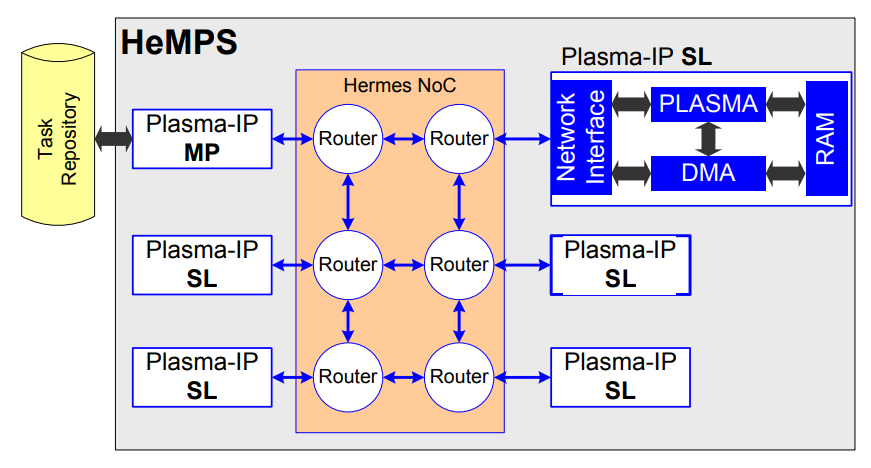
\includegraphics[width=\hsize]{imagens/HeMPS.png}}%
\legend{Aqui entra a legenda da figura. Deve ser simples e sucinto.
Qualquer explicação mais longa deve estar no corpo do texto.}
\source{\cite{bib:hemps}}
\end{figure}

\chapter{Implementação paralelo do PSO}

Executar na Memphis outras funções (esphere, rosenbrock, rastringin)

%----------------------------------------------------------------
\section{Estratégia de paralelismo}
%----------------------------------------------------------------

Texto da seção

%----------------------------------------------------------------
\section{Topologia de comunicação}
%----------------------------------------------------------------

Texto da seção

%----------------------------------------------------------------
\section{Resultados experimentais}
%----------------------------------------------------------------

Nesta seção apresentaremos os resultados das execuções do algoritmo PSO na plataforma Memphis.
A coluna “Nº de elementos processadores” se refere à quantidade do mestre somado aos processadores escravos, exceto ao que se refere com 1 que é o algoritmo serial. Já a coluna “Tempo algoritmo (ticks)” se refere ao tempo de execução do algoritmo somente com o tempo em ticks, cada tick equivale a 10µs. A coluna “Tempo plataforma (ticks)” se refere ao tempo do algoritmo somado ao tempo da preparação da plataforma. A coluna “Speedup”...

Lei de Amdahl

\begin{align}
    &G=\frac{1}{S+\frac{1-S}{n}}
\end{align}

Nas tabelas \ref{cenario1} a \ref{cenario20} estão os valores de cada execução do algoritmo na plataforma Memphis variando a população e as interações:

citando o gráfico \ref{cenario1a5}

%-------------------------------------------------------------------------
%                               TABELAS
%-------------------------------------------------------------------------

%-------------------------------------------------------------------------
%                               20 iterações
%-------------------------------------------------------------------------

\begin{table}[h]{12cm}
    \caption{Cenário de teste com população igual a 100 e 20 iterações}
    \label{cenario1}
    \begin{tabular}{llll}
        \hline
        \shortstack[l]{Nº de elementos \\ processadores} & \shortstack[l]{Tempo algoritmo \\ (ticks)} & \shortstack[l]{Tempo plataforma \\ (ticks)} & Speedup \\
        \hline
        1 & 1.615.530 & 1.617.079 & 1,00 \\
        2 & 1.950.193 & 1.951.735 & 0,83 \\
        3 & 1.024.344 & 1.025.892 &	1,58 \\
        4 & 720.708   & 722.186   & 2,24 \\
        5 & 589.084   & 590.562   & 2,74 \\
        6 & 503.492   & 504.970   & 3,21 \\
        \hline
    \end{tabular}
    %\legend{Texto da legenda. (Opcional)}
    %\source{Citação da fonte ou `O autor'. (opcional)}
\end{table}

\begin{table}[h]{12cm}
    \caption{Cenário de teste com população igual a 200 e 20 iterações}
    \label{cenario2}
    \begin{tabular}{llll}
        \hline
        \shortstack[l]{Nº de elementos \\ processadores} & \shortstack[l]{Tempo algoritmo \\ (ticks)} & \shortstack[l]{Tempo plataforma \\ (ticks)} & Speedup \\
        \hline
        1 & 3.175.949 & 3.177.498 & 1,00 \\
        2 & 3.802.205 & 3.803.747 & 0,84 \\
        3 & 1.951.996 & 1.953.544 &	1,63 \\
        4 & 1.350.049 & 1.351.597 & 2,35 \\
        5 & 1.048.768 & 1.050.316 & 3,03 \\
        6 & 876.873   & 878.351   & 3,62 \\
        \hline
    \end{tabular}
    %\legend{Texto da legenda. (Opcional)}
    %\source{Citação da fonte ou `O autor'. (opcional)}
\end{table}

\begin{table}[h]{12cm}
    \caption{Cenário de teste com população igual a 300 e 20 iterações}
    \label{cenario3}
    \begin{tabular}{llll}
        \hline
        \shortstack[l]{Nº de elementos \\ processadores} & \shortstack[l]{Tempo algoritmo \\ (ticks)} & \shortstack[l]{Tempo plataforma \\ (ticks)} & Speedup \\
        \hline
        1 & 4.732.875 & 4.734.424 & 1,00 \\
        2 & 5.657.594 & 5.659.136 & 0,84 \\
        3 & 2.875.817 & 2.877.365 &	1,65 \\
        4 & 1.960.693 & 1.962.241 & 2,41 \\
        5 & 1.511.697 & 1.513.245 & 3,13 \\
        6 & 1.245.103 & 1.246.651 & 3,80 \\
        \hline
    \end{tabular}
    %\legend{Texto da legenda. (Opcional)}
    %\source{Citação da fonte ou `O autor'. (opcional)}
\end{table}

\begin{table}[h]{12cm}
    \caption{Cenário de teste com população igual a 400 e 20 iterações}
    \label{cenario4}
    \begin{tabular}{llll}
        \hline
        \shortstack[l]{Nº de elementos \\ processadores} & \shortstack[l]{Tempo algoritmo \\ (ticks)} & \shortstack[l]{Tempo plataforma \\ (ticks)} & Speedup \\
        \hline
        1 & 6.281.550 & 6.283.099 & 1,00 \\
        2 & 7.515.159 & 7.516.701 & 0,84 \\
        3 & 3.805.477 & 3.807.025 &	1,65 \\
        4 & 2.574.297 & 2.575.845 & 2,44 \\
        5 & 1.976.616 & 1.978.164 & 3,18 \\
        6 & 1.613.632 & 1.615.180 & 3,89 \\
        \hline
    \end{tabular}
    %\legend{Texto da legenda. (Opcional)}
    %\source{Citação da fonte ou `O autor'. (opcional)}
\end{table}

\begin{table}[h]{12cm}
    \caption{Cenário de teste com população igual a 500 e 20 iterações}
    \label{cenario5}
    \begin{tabular}{llll}
        \hline
        \shortstack[l]{Nº de elementos \\ processadores} & \shortstack[l]{Tempo algoritmo \\ (ticks)} & \shortstack[l]{Tempo plataforma \\ (ticks)} & Speedup \\
        \hline
        1 & 7.844.240 & 7.845.789 & 1,00 \\
        2 & 9.373.217 & 9.374.760 & 0,84 \\
        3 & 4.736.120 & 4.737.668 &	1,66 \\
        4 & 3.202.018 & 3.203.566 & 2,45 \\
        5 & 2.440.490 & 2.442.038 & 3,21 \\
        6 & 1.984.755 & 1.986.303 & 3,95 \\
        \hline
    \end{tabular}
    %\legend{Texto da legenda. (Opcional)}
    %\source{Citação da fonte ou `O autor'. (opcional)}
\end{table}

%-------------------------------------------------------------------------
%                               30 iterações
%-------------------------------------------------------------------------

\begin{table}[h]{12cm}
    \caption{Cenário de teste com população igual a 100 e 30 iterações}
    \label{cenario6}
    \begin{tabular}{llll}
        \hline
        \shortstack[l]{Nº de elementos \\ processadores} & \shortstack[l]{Tempo algoritmo \\ (ticks)} & \shortstack[l]{Tempo plataforma \\ (ticks)} & Speedup \\
        \hline
        1 & 2.391.648 & 2.393.582 & 1,00 \\
        2 & 2.869.352 & 2.870.894 & 0,83 \\
        3 & 1.491.879 & 1.493.427 &	1,60 \\
        4 & 1.035.484 & 1.037.032 & 2,31 \\
        5 & 831.658   & 833.136   & 2,88 \\
        6 & 701.940   & 703.624   & 3,41 \\
        \hline
    \end{tabular}
    %\legend{Texto da legenda. (Opcional)}
    %\source{Citação da fonte ou `O autor'. (opcional)}
\end{table}

\begin{table}[h]{12cm}
    \caption{Cenário de teste com população igual a 200 e 30 iterações}
    \label{cenario7}
    \begin{tabular}{llll}
        \hline
        \shortstack[l]{Nº de elementos \\ processadores} & \shortstack[l]{Tempo algoritmo \\ (ticks)} & \shortstack[l]{Tempo plataforma \\ (ticks)} & Speedup \\
        \hline
        1 & 4.706.089 & 4.707.638 & 1,00 \\
        2 & 5.617.876 & 5.619.418 & 0,84 \\
        3 & 2.867.739 & 2.869.287 &	1,64 \\
        4 & 1.969.392 & 1.970.940 & 2,39 \\
        5 & 1.516.018 & 1.517.566 & 3,10 \\
        6 & 1.254.767 & 1.256.315 & 3,75 \\
        \hline
    \end{tabular}
    %\legend{Texto da legenda. (Opcional)}
    %\source{Citação da fonte ou `O autor'. (opcional)}
\end{table}

\begin{table}[h]{12cm}
    \caption{Cenário de teste com população igual a 300 e 30 iterações}
    \label{cenario8}
    \begin{tabular}{llll}
        \hline
        \shortstack[l]{Nº de elementos \\ processadores} & \shortstack[l]{Tempo algoritmo \\ (ticks)} & \shortstack[l]{Tempo plataforma \\ (ticks)} & Speedup \\
        \hline
        1 & 7.024.437 & 7.025.986 & 1,00 \\
        2 & 8.368.147 & 8.369.689 & 0,84 \\
        3 & 4.238.051 & 4.239.599 &	1,66 \\
        4 & 2.876.310 & 2.877.858 & 2,44 \\
        5 & 2.204.034 & 2.205.582 & 3,19 \\
        6 & 1.802.087 & 1.803.635 & 3,90 \\
        \hline
    \end{tabular}
    %\legend{Texto da legenda. (Opcional)}
    %\source{Citação da fonte ou `O autor'. (opcional)}
\end{table}

\begin{table}[h]{12cm}
    \caption{Cenário de teste com população igual a 400 e 30 iterações}
    \label{cenario9}
    \begin{tabular}{llll}
        \hline
        \shortstack[l]{Nº de elementos \\ processadores} & \shortstack[l]{Tempo algoritmo \\ (ticks)} & \shortstack[l]{Tempo plataforma \\ (ticks)} & Speedup \\
        \hline
        1 & 9.322.725  & 9.324.274  & 1,00 \\
        2 & 11.123.300 & 11.124.922 & 0,84 \\
        3 & 5.617.266  & 5.618.814  & 1,66 \\
        4 & 3.785.258  & 3.786.506  & 2,46 \\
        5 & 2.892.925  & 2.894.473  & 3,22 \\
        6 & 2.349.432  & 2.350.980  & 3,97 \\
        \hline
    \end{tabular}
    %\legend{Texto da legenda. (Opcional)}
    %\source{Citação da fonte ou `O autor'. (opcional)}
\end{table}

\begin{table}[h]{12cm}
    \caption{Cenário de teste com população igual a 500 e 30 iterações}
    \label{cenario10}
    \begin{tabular}{llll}
        \hline
        \shortstack[l]{Nº de elementos \\ processadores} & \shortstack[l]{Tempo algoritmo \\ (ticks)} & \shortstack[l]{Tempo plataforma \\ (ticks)} & Speedup \\
        \hline
        1 & 11.643.190 & 11.644.820 & 1,00 \\
        2 & 13.880.754 & 13.882.376 & 0,84 \\
        3 & 6.995.997  & 6.997.545  & 1,66 \\
        4 & 4.717.449  & 4.718.997  & 2,47 \\
        5 & 3.581.066  & 3.582.614  & 3,25 \\
        6 & 2.900.382  & 2.901.930  & 4,01 \\
        \hline
    \end{tabular}
    %\legend{Texto da legenda. (Opcional)}
    %\source{Citação da fonte ou `O autor'. (opcional)}
\end{table}

%-------------------------------------------------------------------------
%                               40 iterações
%-------------------------------------------------------------------------

\begin{table}[h]{12cm}
    \caption{Cenário de teste com população igual a 100 e 40 iterações}
    \label{cenario11}
    \begin{tabular}{llll}
        \hline
        \shortstack[l]{Nº de elementos \\ processadores} & \shortstack[l]{Tempo algoritmo \\ (ticks)} & \shortstack[l]{Tempo plataforma \\ (ticks)} & Speedup \\
        \hline
        1 & 3.165.517 & 3.167.066 & 1,00 \\
        2 & 3.787.460 & 3.789.002 & 0,84 \\
        3 & 1.958.955 & 1.960.503 &	1,62 \\
        4 & 1.350.337 & 1.351.885 & 2,34 \\
        5 & 1.074.999 & 1.076.547 & 2,94 \\
        6 & 900.399   & 901.877   & 3,52 \\
        \hline
    \end{tabular}
    %\legend{Texto da legenda. (Opcional)}
    %\source{Citação da fonte ou `O autor'. (opcional)}
\end{table}

\begin{table}[h]{12cm}
    \caption{Cenário de teste com população igual a 200 e 40 iterações}
    \label{cenario12}
    \begin{tabular}{llll}
        \hline
        \shortstack[l]{Nº de elementos \\ processadores} & \shortstack[l]{Tempo algoritmo \\ (ticks)} & \shortstack[l]{Tempo plataforma \\ (ticks)} & Speedup \\
        \hline
        1 & 6.235.133 & 6.236.682 & 1,00 \\
        2 & 7.431.111 & 7.432.653 & 0,84 \\
        3 & 3.781.978 & 3.783.526 &	1,65 \\
        4 & 2.588.680 & 2.590.228 & 2,41 \\
        5 & 1.983.270 & 1.984.818 & 3,14 \\
        6 & 1.632.105 & 1.633.653 & 3,82 \\
        \hline
    \end{tabular}
    %\legend{Texto da legenda. (Opcional)}
    %\source{Citação da fonte ou `O autor'. (opcional)}
\end{table}

\begin{table}[h]{12cm}
    \caption{Cenário de teste com população igual a 300 e 40 iterações}
    \label{cenario13}
    \begin{tabular}{llll}
        \hline
        \shortstack[l]{Nº de elementos \\ processadores} & \shortstack[l]{Tempo algoritmo \\ (ticks)} & \shortstack[l]{Tempo plataforma \\ (ticks)} & Speedup \\
        \hline
        1 & 9.310.226  & 9.311.775  & 1,00 \\
        2 & 11.076.869 & 11.078.491 & 0,84 \\
        3 & 5.600.291  & 5.601.839  & 1,66 \\
        4 & 3.790.819  & 3.792.367  & 2,46 \\
        5 & 2.896.281  & 2.897.829  & 3,21 \\
        6 & 2.358.590  & 2.360.138  & 3,95 \\
        \hline
    \end{tabular}
    %\legend{Texto da legenda. (Opcional)}
    %\source{Citação da fonte ou `O autor'. (opcional)}
\end{table}

\begin{table}[h]{12cm}
    \caption{Cenário de teste com população igual a 400 e 40 iterações}
    \label{cenario14}
    \begin{tabular}{llll}
        \hline
        \shortstack[l]{Nº de elementos \\ processadores} & \shortstack[l]{Tempo algoritmo \\ (ticks)} & \shortstack[l]{Tempo plataforma \\ (ticks)} & Speedup \\
        \hline
        1 & 12.361.637 & 12.363.266 & 1,00 \\
        2 & 14.729.113 & 14.730.734 & 0,84 \\
        3 & 7.427.058  & 7.428.606  & 1,66 \\
        4 & 4.995.090  & 4.996.638  & 2,47 \\
        5 & 3.808.108  & 3.809.656  & 3,25 \\
        6 & 3.084.966  & 3.086.514  & 4,01 \\
        \hline
    \end{tabular}
    %\legend{Texto da legenda. (Opcional)}
    %\source{Citação da fonte ou `O autor'. (opcional)}
\end{table}

\begin{table}[h]{12cm}
    \caption{Cenário de teste com população igual a 500 e 40 iterações}
    \label{cenario15}
    \begin{tabular}{llll}
        \hline
        \shortstack[l]{Nº de elementos \\ processadores} & \shortstack[l]{Tempo algoritmo \\ (ticks)} & \shortstack[l]{Tempo plataforma \\ (ticks)} & Speedup \\
        \hline
        1 & 15.439.550 & 15.441.180 & 1,00 \\
        2 & 18.384.023 & 18.385.646 & 0,84 \\
        3 & 9.253.339  & 9.254.887  & 1,67 \\
        4 & 6.232.248  & 6.233.796  & 2,48 \\
        5 & 4.721.028  & 4.722.576  & 3,27 \\
        6 & 3.815.373  & 3.816.921  & 4,05 \\
        \hline
    \end{tabular}
    %\legend{Texto da legenda. (Opcional)}
    %\source{Citação da fonte ou `O autor'. (opcional)}
\end{table}

%-------------------------------------------------------------------------
%                               50 iterações
%-------------------------------------------------------------------------

\begin{table}[h]{12cm}
    \caption{Cenário de teste com população igual a 100 e 50 iterações}
    \label{cenario16}
    \begin{tabular}{llll}
        \hline
        \shortstack[l]{Nº de elementos \\ processadores} & \shortstack[l]{Tempo algoritmo \\ (ticks)} & \shortstack[l]{Tempo plataforma \\ (ticks)} & Speedup \\
        \hline
        1 & 3.939.130 & 3.940.679 & 1,00 \\
        2 & 4.704.341 & 4.708.553 & 0,84 \\
        3 & 2.425.787 & 2.427.335 &	1,62 \\
        4 & 1.665.306 & 1.666.854 & 2,37 \\
        5 & 1.318.249 & 1.319.797 & 2,99 \\
        6 & 1.098.792 & 1.100.340 & 3,58 \\
        \hline
    \end{tabular}
    %\legend{Texto da legenda. (Opcional)}
    %\source{Citação da fonte ou `O autor'. (opcional)}
\end{table}

\begin{table}[h]{12cm}
    \caption{Cenário de teste com população igual a 200 e 50 iterações}
    \label{cenario17}
    \begin{tabular}{llll}
        \hline
        \shortstack[l]{Nº de elementos \\ processadores} & \shortstack[l]{Tempo algoritmo \\ (ticks)} & \shortstack[l]{Tempo plataforma \\ (ticks)} & Speedup \\
        \hline
        1 & 7.763.052 & 7.764.601 & 1,00 \\
        2 & 9.246.037 & 9.247.579 & 0,84 \\
        3 & 4.696.389 & 4.697.937 &	1,65 \\
        4 & 3.207.139 & 3.208.687 & 2,42 \\
        5 & 2.450.316 & 2.451.864 & 3,17 \\
        6 & 2.009.146 & 2.010.694 & 3,86 \\
        \hline
    \end{tabular}
    %\legend{Texto da legenda. (Opcional)}
    %\source{Citação da fonte ou `O autor'. (opcional)}
\end{table}

\begin{table}[h]{12cm}
    \caption{Cenário de teste com população igual a 300 e 50 iterações}
    \label{cenario18}
    \begin{tabular}{llll}
        \hline
        \shortstack[l]{Nº de elementos \\ processadores} & \shortstack[l]{Tempo algoritmo \\ (ticks)} & \shortstack[l]{Tempo plataforma \\ (ticks)} & Speedup \\
        \hline
        1 & 11.594.212 & 11.596.841 & 1,00 \\
        2 & 13.784.014 & 13.785.635 & 0,84 \\
        3 & 6.962.254  & 6.963.802  & 1,67 \\
        4 & 4.705.656  & 4.707.204  & 2,46 \\
        5 & 3.587.669  & 3.589.217  & 3,23 \\
        6 & 2.915.521  & 2.917.069  & 3,98 \\
        \hline
    \end{tabular}
    %\legend{Texto da legenda. (Opcional)}
    %\source{Citação da fonte ou `O autor'. (opcional)}
\end{table}

\begin{table}[h]{12cm}
    \caption{Cenário de teste com população igual a 400 e 50 iterações}
    \label{cenario19}
    \begin{tabular}{llll}
        \hline
        \shortstack[l]{Nº de elementos \\ processadores} & \shortstack[l]{Tempo algoritmo \\ (ticks)} & \shortstack[l]{Tempo plataforma \\ (ticks)} & Speedup \\
        \hline
        1 & 15.399.723 & 15.401.352 & 1,00 \\
        2 & 18.332.980 & 18.334.601 & 0,84 \\
        3 & 9.237.387  & 9.238.935  & 1,67 \\
        4 & 6.205.400  & 6.206.948  & 2,48 \\
        5 & 4.723.163  & 4.724.711  & 3,26 \\
        6 & 3.820.284  & 3.821.832  & 4,03 \\
        \hline
    \end{tabular}
    %\legend{Texto da legenda. (Opcional)}
    %\source{Citação da fonte ou `O autor'. (opcional)}
\end{table}

\begin{table}[h]{12cm}
    \caption{Cenário de teste com população igual a 500 e 50 iterações}
    \label{cenario20}
    \begin{tabular}{llll}
        \hline
        \shortstack[l]{Nº de elementos \\ processadores} & \shortstack[l]{Tempo algoritmo \\ (ticks)} & \shortstack[l]{Tempo plataforma \\ (ticks)} & Speedup \\
        \hline
        1 & 19.235.575 & 19.237.202 & 1,00 \\
        2 & 22.885.567 & 22.887.187 & 0,84 \\
        3 & 11.510.217 & 11.511.845 & 1,67 \\
        4 & 7.746.771  & 7.748.319  & 2,48 \\
        5 & 5.860.508  & 5.862.056  & 3,28 \\
        6 & 4.730.160  & 4.731.708  & 4,07 \\
        \hline
    \end{tabular}
    %\legend{Texto da legenda. (Opcional)}
    %\source{Citação da fonte ou `O autor'. (opcional)}
\end{table}

%-------------------------------------------------------------------------
%                               GRÁFICOS
%-------------------------------------------------------------------------

\begin{graph}[h]{16cm}
    \caption{Cenário de teste com 20 iterações}
    \label{cenario1a5}
        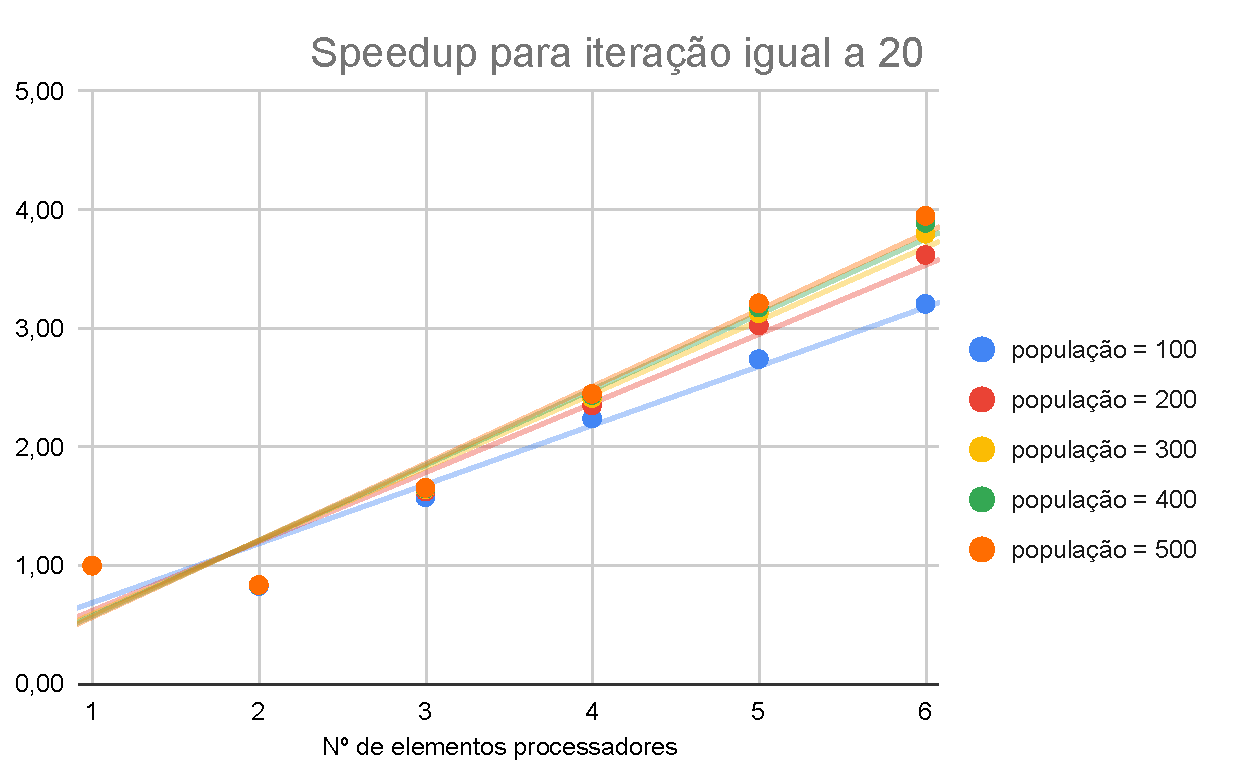
\includegraphics[width=14cm]{graficos/Speedup para iteração igual a 20.pdf}
\end{graph}

\begin{graph}[h]{16cm}
    \caption{Cenário de teste com 30 iterações}
    \label{cenario6a10}
        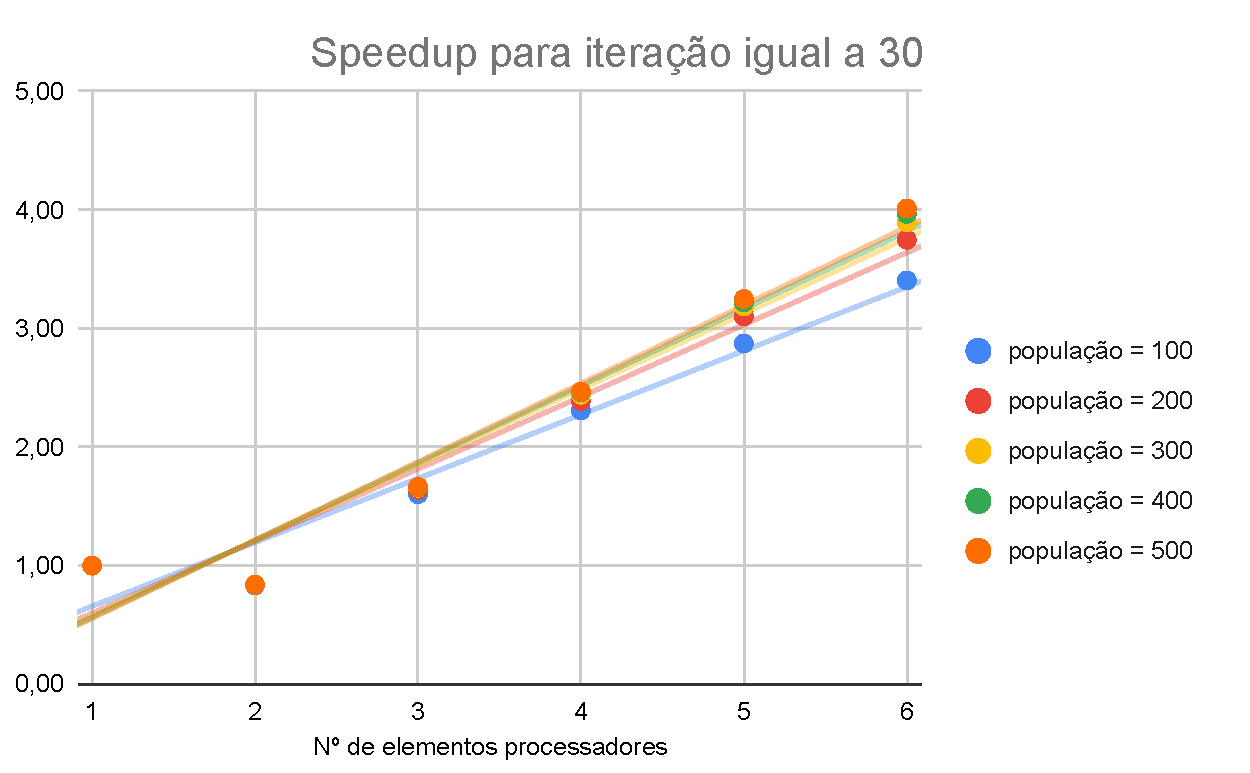
\includegraphics[width=14cm]{graficos/Speedup para iteração igual a 30.pdf}
\end{graph}

\begin{graph}[h]{16cm}
    \caption{Cenário de teste com 40 iterações}
    \label{cenario11a15}
        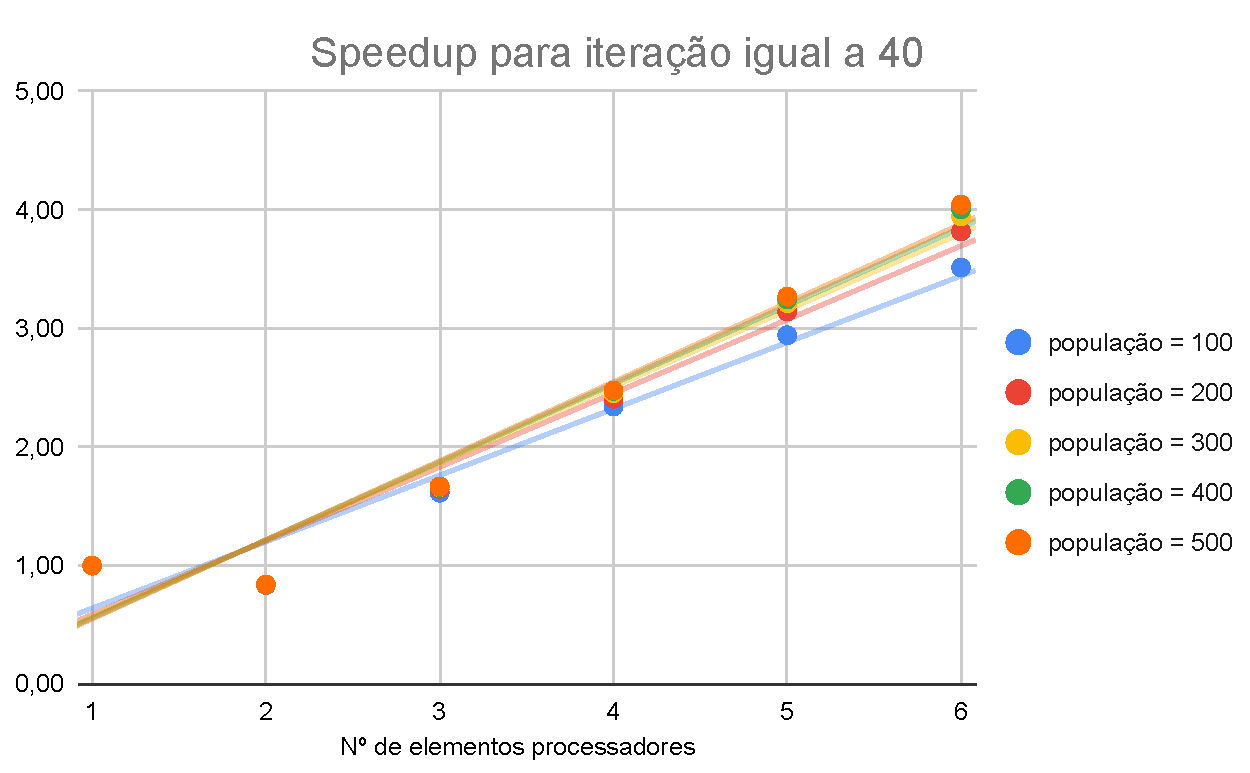
\includegraphics[width=14cm]{graficos/Speedup para iteração igual a 40.pdf}
\end{graph}

\begin{graph}[h]{16cm}
    \caption{Cenário de teste com 50 iterações}
    \label{cenario16a20}
    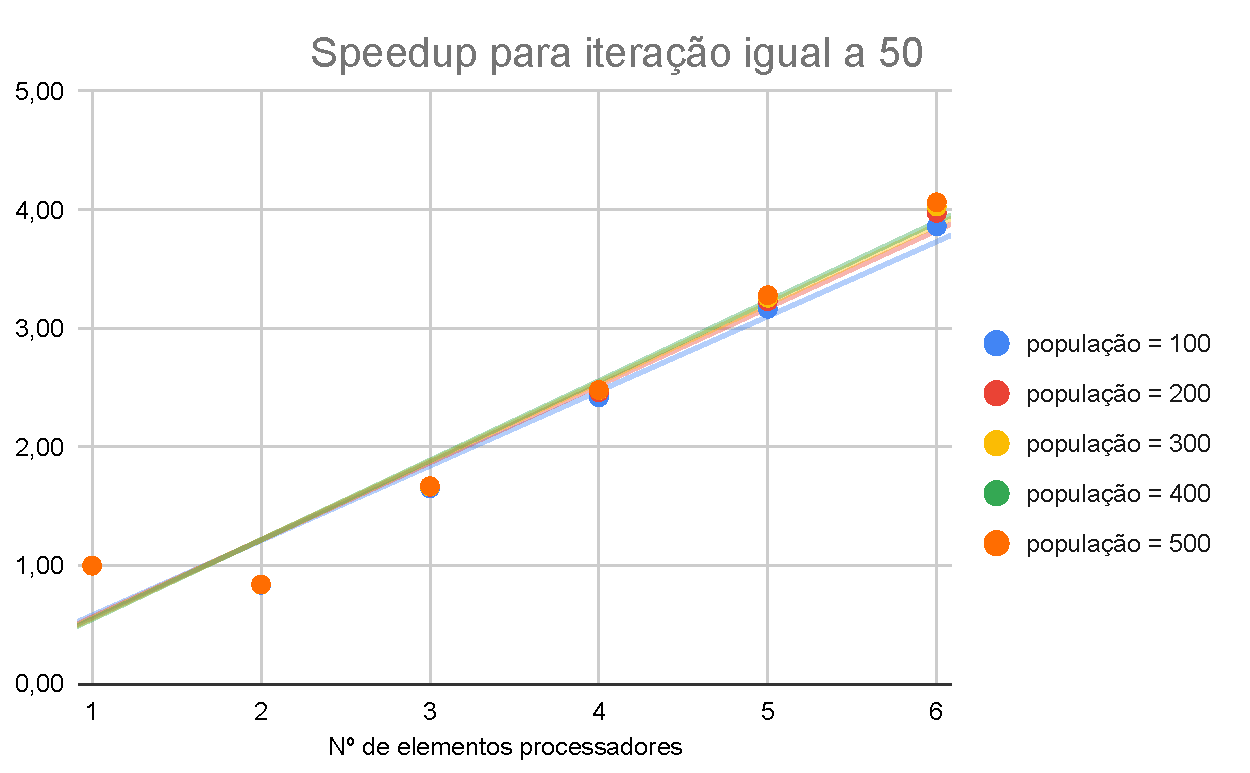
\includegraphics[width=14cm]{graficos/Speedup para iteração igual a 50.pdf}
\end{graph}

%\begin{figure}[ht]{12cm}
%  \begin{center}
%    \leavevmode
%    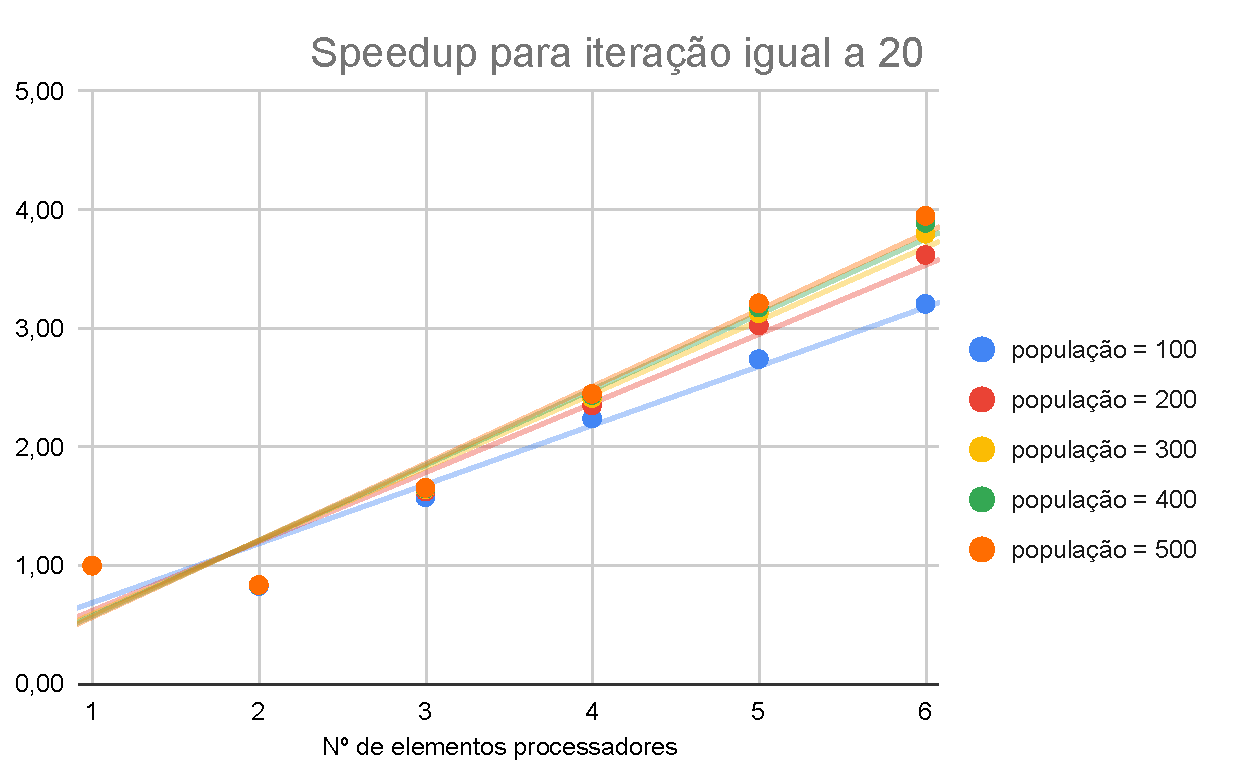
\includegraphics[width=0.65\textwidth]{graficos/Speedup para iteração igual a 20.pdf}
%    \caption{Two element linear array (from \cite{gross15})}
%    \label{fig:2elem}
%  \end{center}
%\end{figure}

%----------------------------------------------------------------
\subsection{Título da subseção}
%----------------------------------------------------------------

Texto da subseção

%----------------------------------------------------------------
\subsubsection{Título da subsubseção}
%----------------------------------------------------------------

Texto da subsubseção

%================================================================
\chapter*{Conclusão}
%================================================================

Texto da conclusão.

%\index{Introdução!Capítulo}.

%XXXXXXXXXXXXXXXXXXXXXXXXXXXXXXXXXXXXXXXXXXXXXXXXXXXXXXXXXXXXXXXX
% ELEMENTOS POS-TEXTUAIS
%XXXXXXXXXXXXXXXXXXXXXXXXXXXXXXXXXXXXXXXXXXXXXXXXXXXXXXXXXXXXXXXX
\backmatter % inicia a área dos elementos pós-textuais
%XXXXXXXXXXXXXXXXXXXXXXXXXXXXXXXXXXXXXXXXXXXXXXXXXXXXXXXXXXXXXXXX

%===========================================================
% Referencias via BibTeX
%===========================================================

\citeoption{abnt-options4}
\bibliography{abnt-options4,bibliografia}
% \bibliographystyle{abntex2-num}
% \bibliography{bibliografia}

%===========================================================
\postextualchapter*{Glossário} % elemento opcional
%===========================================================

\definicao{termo 1}{significado}
\definicao{termo 2}{significado}
\definicao{termo 3}{significado}

%XXXXXXXXXXXXXXXXXXXXXXXXXXXXXXXXXXXXXXXXXXXXXXXXXXXXXXXXXXX
% Apêndices (opcionais)
%XXXXXXXXXXXXXXXXXXXXXXXXXXXXXXXXXXXXXXXXXXXXXXXXXXXXXXXXXXX
\appendix % inicia os apêndices
%XXXXXXXXXXXXXXXXXXXXXXXXXXXXXXXXXXXXXXXXXXXXXXXXXXXXXXXXXXX

%===========================================================
\postextualchapter{Primeiro apêndice}
%===========================================================

% ----------------------------------------------------------
\section{Primeira seção}
% ----------------------------------------------------------

Texto da primeira seção.

% ----------------------------------------------------------
\subsection{Primeira subseção}
% ----------------------------------------------------------

Texto da primeira subseção.

% ----------------------------------------------------------
\subsubsection{Primeira subsubseção}
% ----------------------------------------------------------

Texto da primeira subsubseção.

%===========================================================
\postextualchapter{Segundo apêndice}
%===========================================================

% ----------------------------------------------------------
\section{Primeira seção}
% ----------------------------------------------------------

Texto da primeira seção.

% ----------------------------------------------------------
\subsection{Primeira subseção}
% ----------------------------------------------------------

Texto da primeira subseção.

% ----------------------------------------------------------
\subsubsection{Primeira subsubseção}
% ----------------------------------------------------------

Texto da primeira subsubseção.

%XXXXXXXXXXXXXXXXXXXXXXXXXXXXXXXXXXXXXXXXXXXXXXXXXXXXXXXXXXX
% Anexos (opcionais)
%XXXXXXXXXXXXXXXXXXXXXXXXXXXXXXXXXXXXXXXXXXXXXXXXXXXXXXXXXXX
\annex % inicia os anexos
%XXXXXXXXXXXXXXXXXXXXXXXXXXXXXXXXXXXXXXXXXXXXXXXXXXXXXXXXXXX

%===========================================================
\postextualchapter{Primeiro anexo}
%===========================================================

% ----------------------------------------------------------
\section{Primeira seção}
% ----------------------------------------------------------

Texto da primeira seção.

% ----------------------------------------------------------
\subsection{Primeira subseção}
% ----------------------------------------------------------

Texto da primeira subseção.

% ----------------------------------------------------------
\subsubsection{Primeira subsubseção}
% ----------------------------------------------------------

Texto da primeira subsubseção.

%===========================================================
\postextualchapter{Segundo anexo}
%===========================================================

% ----------------------------------------------------------
\section{Primeira seção}
% ----------------------------------------------------------

Texto da primeira seção.

% ----------------------------------------------------------
\subsection{Primeira subseção}
% ----------------------------------------------------------

Texto da primeira subseção.

% ----------------------------------------------------------
\subsubsection{Primeira subsubseção}
% ----------------------------------------------------------

Texto da primeira subsubseção.

%/\/\/\/\/\/\/\/\/\/\/\/\/\/\/\/\/\/\/\/\/\/\/\/\/\/\/\/\/\/
\end{document}
%/\/\/\/\/\/\/\/\/\/\/\/\/\/\/\/\/\/\/\/\/\/\/\/\/\/\/\/\/\/